\documentclass[oneside,openany,headings=optiontotoc,11pt,numbers=noenddot]{scrreprt}

\usepackage[a4paper]{geometry}
\usepackage[utf8]{inputenc}
\usepackage[T1]{fontenc}
\usepackage{lmodern}
\usepackage[ngerman]{babel}
\usepackage{ngerman}

\usepackage[onehalfspacing]{setspace}

\usepackage{fancyhdr}
\usepackage{fancybox}

\usepackage{rotating}
\usepackage{varwidth}

%Struktogramme
\usepackage[german,curves]{struktex}

\usepackage{pdflscape}
\usepackage{changepage}
\usepackage{graphicx}
\usepackage[bottom]{footmisc}
\usepackage{transparent}
\usepackage{graphbox}
\graphicspath{
	{Pics/PDFs/}
	{Pics/JPGs/}
	{Pics/PNGs/}
}
\usepackage{caption}
\usepackage{wrapfig}
\usepackage{marginnote}
\usepackage{tabularx}
\usepackage{dashrule}
\usepackage{soulutf8}
\usepackage{hhline}
%arydshln suppresses vertical lines in table
%\usepackage{arydshln}
\usepackage{multirow}
\usepackage{enumerate}
\usepackage[hidelinks]{hyperref}
\usepackage{listings}

\usepackage[table]{xcolor}
\usepackage{array}
\usepackage{enumitem,amssymb,amsmath}
\usepackage{interval}
\usepackage{cancel}
\usepackage{stmaryrd}
\usepackage{wasysym}
\usepackage{polynom}
\usepackage{diagbox}
\usepackage{dashrule}
\usepackage{framed}
\usepackage{mdframed}
\usepackage{karnaugh-map}
\usepackage{pdfpages}

\usepackage{blindtext}

\usepackage{eso-pic}

\usepackage{amssymb}
\usepackage{eurosym}

\usepackage[pages=some]{background}
\pagestyle{headings}
\renewcommand{\headrulewidth}{0.2pt}
\renewcommand{\footrulewidth}{0.2pt}
\newcommand*{\underdownarrow}[2]{\ensuremath{\underset{\overset{\Big\downarrow}{#2}}{#1}}}
\setlength{\fboxsep}{5pt}
\newcommand{\explainBelow}[3]{\underbrace{#1}_{\parbox{\widthof{#3}}{\footnotesize\raggedright #2}}}
\newcommand{\explainAbove}[3]{\overbrace{#1}^{\parbox{\widthof{#3}}{\footnotesize\raggedright #2}}}
\newcommand\footnoteref[1]{\protected@xdef\@thefnmark{\ref{#1}}\@footnotemark}


% Codestyle defined
\definecolor{codegreen}{rgb}{0,0.6,0}
\definecolor{codegray}{rgb}{0.5,0.5,0.5}
\definecolor{codepurple}{rgb}{0.58,0,0.82}
\definecolor{backcolour}{rgb}{0.95,0.95,0.92}
\definecolor{deepgreen}{rgb}{0,0.5,0}
\definecolor{darkblue}{rgb}{0,0,0.65}
\definecolor{mauve}{rgb}{0.40, 0.19,0.28}
\colorlet{exceptioncolour}{yellow!50!red}
\colorlet{commandcolour}{blue!60!black}
\colorlet{numpycolour}{blue!60!green}
\colorlet{specmethodcolour}{violet}

%Neue Spaltendefinition
\newcolumntype{L}[1]{>{\raggedright\let\newline\\\arraybackslash\hspace{0pt}}m{#1}}
\newcolumntype{M}{>{\centering\arraybackslash}X}
\newcommand{\cmnt}[1]{\ignorespaces}
%Textausrichtung ändern
\newcommand\tabrotate[1]{\rotatebox{90}{\raggedright#1\hspace{\tabcolsep}}}

%Intervall-Konfig
\intervalconfig {
	soft open fences
}

%Bash
\lstdefinestyle{BashInputStyle}{
	language=bash,
	basicstyle=\small\sffamily,
	backgroundcolor=\color{backcolour},
	columns=fullflexible,
	backgroundcolor=\color{backcolour},
	breaklines=true,
}
%Java
\lstdefinestyle{JavaInputStyle}{
	language=Java,
	backgroundcolor=\color{backcolour},
	aboveskip=1mm,
	belowskip=1mm,
	showstringspaces=false,
	columns=flexible,
	basicstyle={\footnotesize\ttfamily},
	numberstyle={\tiny},
	numbers=none,
	keywordstyle=\color{purple},,
	commentstyle=\color{deepgreen},
	stringstyle=\color{blue},
	emph={out},
	emphstyle=\color{darkblue},
	emph={[2]rand},
	emphstyle=[2]\color{specmethodcolour},
	breaklines=true,
	breakatwhitespace=true,
	tabsize=2,
}
%Python
\lstdefinestyle{PythonInputStyle}{
	language=Python,
	alsoletter={1234567890},
	aboveskip=1ex,
	basicstyle=\footnotesize,
	breaklines=true,
	breakatwhitespace= true,
	backgroundcolor=\color{backcolour},
	commentstyle=\color{red},
	otherkeywords={\ , \}, \{, \&,\|},
	emph={and,break,class,continue,def,yield,del,elif,else,%
		except,exec,finally,for,from,global,if,import,in,%
		lambda,not,or,pass,print,raise,return,try,while,assert},
	emphstyle=\color{exceptioncolour},
	emph={[2]True,False,None,min},
	emphstyle=[2]\color{specmethodcolour},
	emph={[3]object,type,isinstance,copy,deepcopy,zip,enumerate,reversed,list,len,dict,tuple,xrange,append,execfile,real,imag,reduce,str,repr},
	emphstyle=[3]\color{commandcolour},
	emph={[4]ode, fsolve, sqrt, exp, sin, cos, arccos, pi,  array, norm, solve, dot, arange, , isscalar, max, sum, flatten, shape, reshape, find, any, all, abs, plot, linspace, legend, quad, polyval,polyfit, hstack, concatenate,vstack,column_stack,empty,zeros,ones,rand,vander,grid,pcolor,eig,eigs,eigvals,svd,qr,tan,det,logspace,roll,mean,cumsum,cumprod,diff,vectorize,lstsq,cla,eye,xlabel,ylabel,squeeze},
	emphstyle=[4]\color{numpycolour},
	emph={[5]__init__,__add__,__mul__,__div__,__sub__,__call__,__getitem__,__setitem__,__eq__,__ne__,__nonzero__,__rmul__,__radd__,__repr__,__str__,__get__,__truediv__,__pow__,__name__,__future__,__all__},
	emphstyle=[5]\color{specmethodcolour},
	emph={[6]assert,range,yield},
	emphstyle=[6]\color{specmethodcolour}\bfseries,
	emph={[7]Exception,NameError,IndexError,SyntaxError,TypeError,ValueError,OverflowError,ZeroDivisionError,KeyboardInterrupt},
	emphstyle=[7]\color{specmethodcolour}\bfseries,
	emph={[8]taster,send,sendMail,capture,check,noMsg,go,move,switch,humTem,ventilate,buzz},
	emphstyle=[8]\color{blue},
	keywordstyle=\color{blue}\bfseries,
	rulecolor=\color{black!40},
	showstringspaces=false,
	stringstyle=\color{deepgreen}
}

\lstset{literate=%
	{Ö}{{\"O}}1
	{Ä}{{\"A}}1
	{Ü}{{\"U}}1
	{ß}{{\ss}}1
	{ü}{{\"u}}1
	{ä}{{\"a}}1
	{ö}{{\"o}}1
}

% Neue Klassenarbeits-Umgebung
\newenvironment{worksheet}[3]
% Begin-Bereich
{
	\newpage
	\sffamily
	\setcounter{page}{1}
	\ClearShipoutPicture
	\AddToShipoutPicture{
		\put(55,761){{
				\mbox{\parbox{385\unitlength}{\tiny \color{codegray}BBS I Mainz, #1 \newline #2
						\newline #3
					}
				}
			}
		}
		\put(455,761){{
				\mbox{\hspace{0.3cm}
\includegraphics[width=0.2\textwidth]{../../logo.pdf}}
			}
		}
	}
}
% End-Bereich
{
	\clearpage
	\ClearShipoutPicture
}

\geometry{left=2.50cm,right=2.50cm,top=3.00cm,bottom=1.00cm,includeheadfoot}

\begin{document}
	\begin{worksheet}{BGY 16}{Mathematik - Lernbereich 3, Algebraisierung}{Hausaufgabe zur Gegenseitigen Lage von Geraden im Raum}
		
		\begin{framed}
			\noindent
			\tiny{\color{codegray}Geradengleichung aufstellen}\\
			\normalsize
			\noindent
			\underline{Aufgabe 1}\\(a) Geben Sie die Gerade durch \(A(4|2|-1)\) und \(B(10|-8|9)\) an.\\
			Wir benötigen einen \textbf{Stützvektor}. Hierfür wählen wir den Ortsvektor zu einem der beiden Punkte. Der Richtungsvektor muss dann von unserem gewählten Punkt ausgehen.\\
			\begin{tabularx}{\textwidth}{XX}
				Stützvektor: \(\vec{0A} = \left(\begin{array}{c}4\\2\\-1\end{array}\right)\) & \(\vec{AB} = \vec{B} - \vec{A} = \left(\begin{array}{c}6\\-10\\10\end{array}\right)\)
			\end{tabularx}
			Die zugehörige Geradengleichung lautet: \[g: \vec{x} =  \left(\begin{array}{c}4\\2\\-1\end{array}\right) + r*\left(\begin{array}{c}6\\-10\\10\end{array}\right)\]\\
			\noindent
			(b) Bestimmen Sie die Gerade mit dem \textbf{Richtungsvektor} \(\left(\begin{array}{c}-6\\8\\-8\end{array}\right)\) so, dass diese durch den Punkt \(B(10|-8|9)\) verläuft.\\
			Da wir den \textbf{Richtungsvektor} bereits gegeben haben, benötigen wir nur noch den \textbf{Stützvektor}. Für diesen verwenden wir den angegebenen Punkt. So ergibt sich die Geradengleichung:
			\[g: \vec{x} = \left(\begin{array}{c}10\\-8\\9\end{array}\right) + r*\left(\begin{array}{c}-6\\8\\-8\end{array}\right)\]\\
			\noindent
			(c) Geben Sie eine Gerade an, die durch den Punkt \(C(4|0|1)\) geht und den \textbf{Stützvektor} \(\left(\begin{array}{c}4\\2\\-1\end{array}\right)\) hat.\\
			Da wir den Stützvektor gegeben haben, benötigen wir noch den \textbf{Richtungsvektor}. Dieser muss von dem Punkt ausgehen, der uns durch den Stützvektor gegeben ist. Somit gilt \[\vec{SC} = \vec{B} - \vec{S} = \left(\begin{array}{c}0\\-2\\2\end{array}\right)\]\\
			Damit erhalten wir die Geradengleichung \(g:\vec{x} = \left(\begin{array}{c}4\\2\\-1\end{array}\right) + r*\left(\begin{array}{c}0\\-2\\2\end{array}\right)\)
		\end{framed}
		\begin{framed}
			\tiny{\color{codegray}Punktprüfung und weiterer Punkt auf einer Geraden}\\
			\normalsize\normalcolor
			\underline{Aufgabe 2}\\
			(a) Gegeben ist \(g:\vec{x} = \left(\begin{array}{c}5\\5\\1\end{array}\right) + r*\left(\begin{array}{c}1\\2\\0\end{array}\right)\).\\
			\(\circ\) Geben Sie zwei Punkte auf der Geraden an. Prüfen Sie zudem, ob die Punkte \(P_1(7|9|1)\) und \(P_2(3|1|0)\) auf \(g\) liegen.\\
			Hierfür wählen wir für \(r\) zwei Werte.\\
			\par\bigskip\noindent
			\begin{tabularx}{\textwidth}{X|X}
				\(r=-2\) & \(r=3\)\\
				\hline
				\(\vec{x} = \left(\begin{array}{c}5\\5\\1\end{array}\right) + (-2)*\left(\begin{array}{c}1\\2\\0\end{array}\right)\) & \(\vec{x} = \left(\begin{array}{c}5\\5\\1\end{array}\right) + 3*\left(\begin{array}{c}1\\2\\0\end{array}\right)\)\\
				\(\vec{x} = \left(\begin{array}{c}3\\1\\1\end{array}\right)\) & \(\vec{x} = \left(\begin{array}{c}8\\11\\1\end{array}\right)\)\\
				\underline{\(A(3|1|1)\)} & \underline{\(B(8|11|1)\)}
			\end{tabularx}\\
			\par\bigskip\noindent
			Für die Punktprüfung setzen wir die Punkte mit der Geradengleichung gleich und prüfen, ob es eine Lösung gibt.\\
			\begin{tabularx}{\textwidth}{X|X}
				\(P_1(7|9|1)\) & \(P_2(3|1|0)\)\\
				\hline
				\(\left(\begin{array}{c}7\\9\\1\end{array}\right) = \left(\begin{array}{c}5\\5\\1\end{array}\right) + r*\left(\begin{array}{c}1\\2\\0\end{array}\right)\) & \(\left(\begin{array}{c}3\\1\\0\end{array}\right) = \left(\begin{array}{c}5\\5\\1\end{array}\right) + r*\left(\begin{array}{c}1\\2\\0\end{array}\right)\)\\
				\par\noindent
				\begin{tabular}{ll}
					\(7=5 +r\) & \(| -5\)\\
					\(9=5+2r\) & \(|-5\)\\
					\(1=1+0r\) & 
				\end{tabular} &
				\begin{tabular}{ll}
					\(3=5 +r\) & \(| -3\)\\
					\(1=5+2r\) & \(|-5\)\\
					\(0=1+0r\) & \(\lightning\)
				\end{tabular}\\
				\cline{1-1}
				\begin{tabular}{lll}
					\(2=r\) \\
					\(4 = 2r\) & \(|:2\) & \(\Rightarrow r = 2\)\\
					\(1=1\) & Wahre Aussage!
				\end{tabular} & \\
				Der Punkt \(P_1\) liegt auf \(g\). & Der Punkt \(P_2\) liegt nicht auf \(g\).
			\end{tabularx}
			\newpage
			(b) Gegeben ist \(h:\vec{x} = \left(\begin{array}{c}2\\3\\4\end{array}\right) + r*\left(\begin{array}{c}0\\1\\-1\end{array}\right)\).\\
			Geben Sie einen Punkt auf der Geraden an. \\
			Um einen Punkt zu bestimmen, wählen wir für \(r\) einen Werte.\\
			\par\bigskip\noindent
			\begin{tabularx}{\textwidth}{X}
				\(r=2\)\\
				\hline
				\(\vec{x} = \left(\begin{array}{c}2\\3\\4\end{array}\right) + 2*\left(\begin{array}{c}0\\1\\-1\end{array}\right)\) \\
				\(\vec{x} = \left(\begin{array}{c}2\\5\\2\end{array}\right)\)\\
				\underline{\(A(2|5|2)\)}
			\end{tabularx}
		\end{framed}
		\begin{framed}
			\noindent
			\tiny{\color{codegray}Grundlagen Vektorrechnung - Geradengleichung}\\
			\normalsize\normalcolor
			\underline{Aufgabe 3}\\
			Das Dreieck ist gegeben durch die Punkte \(A(2|0|3), B(1|-1|5)\) und \(C(3|-2|0)\).\\
			\par\bigskip\noindent
			(a) Bestimmen Sie den Winkel im Punkt C.\\
			\par\noindent
			Um den Winkel im Punkt C zu bestimmen, benötigen wir die von C ausgehenden Vektoren \(\vec{CA}\) und \(\vec{CB}\).\\
			Zusätzlich benötigen wir die Länge der Vektoren.\\
			\begin{tabularx}{\textwidth}{XX}
				\(\vec{CA} = \vec{A} - \vec{C} = \left(\begin{array}{c}-1\\2\\3\end{array}\right)\) & \(\vec{CB} = \vec{B} - \vec{C} = \left(\begin{array}{c}-2\\1\\5\end{array}\right)\)\\
				Länge & Länge
			\end{tabularx}\\
			\par\noindent
			Mit der Umkehrfunktion \[\gamma = \arccos\left(\frac{\vec{a}*\vec{b}}{|\vec{a}|*|\vec{b}|}\right) = \left(\frac{a_1*b_1 + a_2*b_2 + a_3*b_3}{\sqrt{a_1^2 + a_2^2 + a_3^2}*\sqrt{b_1^2 + b_2^2 + b_3^2}}\right)\] bestimmen wir den Winkel im Punkt C.\\
			\[\arccos\left(\frac{(-1)*(-2) + 2*1 + 3*5}{\sqrt{(-1)^2+2^2+3^2}*\sqrt{(-2)^2+1^2+5^2}}\right) = \arccos\left(\frac{19}{\sqrt{14}*\sqrt{30}}\right) = \underline{22,01^\circ}\]
			(b)\\
			\small{\textbf{\color{red}Bitte beachten: Die im Unterricht angegebene Aufgabe (Dienstag und Freitag) war fehlerhaft (bzw. die Strecke lag nicht auf der Geraden g). Es folgt eine verbesserte Variante - mit \underline{angepasster Geraden}!}}\\
			\normalcolor\normalsize
			Wir bezeichnen den Mittelpunkt zwischen A und B mit \(M\). Zeigen Sie, dass die Strecke \(\overline{MC}\) auf \(g: \vec{x} = \left(\begin{array}{c}9\\-5\\-8\end{array}\right) + r*\left(\begin{array}{c}-5\\3\\8\end{array}\right)\) liegt.\\
			\par\bigskip\noindent
			Zunächst bestimmen wir den Mittelpunkt zwischen den Punkten A und B. Hierfür betrachten wir jede Punktkoordinate einzeln. \[M =(m_1|m_2|m_3) = \left(\frac{a_1+b_1}{2}|\frac{a_2+b_2}{2}|\frac{a_3+b_3}{2}\right) = \left(-1.5|1.5|4\right)\]
			Da eine Strecke immer Teil einer Geraden ist, werden wir zur Lösung der Aufgabe zeigen, dass die Gerade \(h\), welche durch die Punkte M und C verläuft, mit der Geraden \(g\) gleich ist.\\
			Zunächst stellen wir also die Geradengleichung durch M und C auf.\\
			\begin{tabularx}{\textwidth}{XX}
				Stützvektor \(\vec{0M} = \left(\begin{array}{c}1.5\\-0.5\\4\end{array}\right)\) & Richtungsvektor \(\vec{MC} = \vec{C}\vec{M} = \left(\begin{array}{c}2.5\\-1.5\\-4\end{array}\right)\)\\
				\multicolumn{2}{c}{\(\Rightarrow h: \vec{x} = \left(\begin{array}{c}1.5\\-0.5\\4\end{array}\right) + t*\left(\begin{array}{c}2.5\\-1.5\\-4\end{array}\right)\)}
			\end{tabularx}
			Bleibt zu zeigen, dass die Geraden \(g\) und \(h\) gleich sind. Hierfür setzen wir \(g=h\) und lösen das entstehende System.\\
			\begin{tabularx}{\textwidth}{rXl}
				I & \(9 -5r = 1.5+2.5t\) & \(\)\\
				II & \(-5+3r = -0.5-1.5t\) & \\
				III & \(-8+8r = 4 -4t\) & \(|-4\ | :(-4)\)\\
				& & \(\xrightarrow{(*)} t = 3-2r\)\\
				\hline\\
			\end{tabularx}
			Wir setzen nun (*) in die Gleichungen I und II ein.\\
			\begin{tabularx}{\textwidth}{rXl}
				I* & \(9 -5r = 1.5+2.5*(3-2r)\)\\
				& \(9-5r = \underbrace{1.5+7.5}_{9} -5r\) & \(|-9 |+5r\)\\
				& \(0 = 0\) & \(\Rightarrow\) Wahre Aussage!\\
				\hline\\
				II* & \(-5+3r = -0.5-1.5*(3-2r)\) & \\
				& \(-5+3r = \underbrace{-0.5-4.5}_{-5} +3r\) & \(| +5 | -3r\)\\
				& \(0 = 0\) & \(\Rightarrow\) Wahre Aussage!
			\end{tabularx}
			Da wir nur \underline{wahre Aussasgen} erhalten, wenn wir das Gleichungssystem lösen, können wir folgern, dass es \underline{\textbf{unendlich viele}} Lösungen für das Gleichungssystem gibt, unsere Geraden also \color{codegreen}gleich\normalcolor.
		\end{framed}
		\begin{framed}
			\noindent
			\tiny{\color{codegray}Geraden so aufstellen, dass sie sich schneiden}\\
			\normalsize\normalcolor
			\noindent
			\underline{Aufgabe 4}\\
			Gegeben ist die Gerade \(g: \vec{x} = \left(\begin{array}{c}3\\1\\7\end{array}\right) + r*\left(\begin{array}{c}2\\-2\\1\end{array}\right)\).\\
			Bestimmen Sie zwei verschiedene Geraden \(h_1\) und \(h_2\), die beide durch den Punkt \(P(2|0|1)\) gehen und orthogonal zu \(g\) liegen.\\
			\par\bigskip\noindent
			Zunächst bestimmen wir den \textbf{Stützvektor} auf. Da sowohl \(h_1\) als auch \(h_2\) durch den Punkt \(P(2|0|1)\) gehen sollen, wählen wir dessen Ortsvektor als Stützvektor.\\
			\begin{tabularx}{\textwidth}{XX}
				\(\vec{p_1} = \vec{0P} = \left(\begin{array}{c}2\\0\\1\end{array}\right)\) & \(\vec{p_2} = \vec{0P} = \left(\begin{array}{c}2\\0\\1\end{array}\right)\)
			\end{tabularx}\\
			Wir erinnern uns:
			\begin{framed}
				\noindent
				Zwei Vektoren \(\vec{a}\) und \(\vec{b}\) sind orthogonal (\(\vec{a}\perp\vec{b}\)), wenn ihr Skalarprodukt Null ist (\(\vec{a}*\vec{b} = 0\)).
			\end{framed}
			\begin{framed}
				\noindent
				Zwei Geraden \(g:\vec{x} = \vec{p} + r*\vec{u}\) und \(h: \vec{x} = \vec{q} + t*\vec{v}\) sind orthogonal zueinander, wenn ihre Richtungsvektoren \(\vec{u}\) und \(\vec{v}\) orthogonal zueinander sind (\(\vec{u}*\vec{v} = 0\)).
			\end{framed}
			\noindent
			Wir benötigen zur Lösung zwei \underline{\textbf{verschiedene} Richtungsvektoren}.\\
			\begin{tabularx}{\textwidth}{X|X}
				\underline{Gesucht}: Richtungsvektor \(\vec{u}\), der orthogonal zu \(\left(\begin{array}{c}2\\-2\\1\end{array}\right)\) ist. & \underline{Gesucht}: Richtungsvektor \(\vec{v}\), mit \(\vec{v} \neq \vec{u}\) und der ist orthogonal zu \(\vec{w} = \left(\begin{array}{c}2\\-2\\1\end{array}\right)\).\\
				\par\noindent
				\(\vec{u}*\vec{w} = u_1*\underbrace{2}_{w_1}+u_2*\underbrace{(-2)}_{w_2}+u_3*\underbrace{1}_{w_3} = 0\) & 				\(\vec{v}*\vec{w} = v_1*\underbrace{2}_{w_1}+v_2*\underbrace{(-2)}_{w_2}+v_3*\underbrace{1}_{w_3} = 0\)\\
				\(\vec{u}*\vec{w} = 1*\underbrace{2}_{w_1}+1*\underbrace{(-2)}_{w_2}+0*\underbrace{1}_{w_3} = 2 - 2 = 0\) & 				\(\vec{v}*\vec{w} = \frac{1}{2}*\underbrace{2}_{w_1}+0*\underbrace{(-2)}_{w_2}+(-1)*\underbrace{1}_{w_3} = 1 - 1 = 0\)\\
				\par\noindent
				\(\vec{u} = \left(\begin{array}{c}1\\1\\0\end{array}\right)\) & \(\vec{v} = \left(\begin{array}{c}\frac{1}{2}\\0\\-1\end{array}\right)\)
			\end{tabularx}
			\newpage
			\noindent
			Wir haben somit zwei verschiedene Richtungsvektoren und können die Geradengleichungen aufstellen:\\
			\begin{tabularx}{\textwidth}{XX}
				\(h_1: \vec{x} = \left(\begin{array}{c}2\\0\\1\end{array}\right) + s*\left(\begin{array}{c}1\\1\\0\end{array}\right)\) & \(h_2: \vec{x} = \left(\begin{array}{c}2\\0\\1\end{array}\right) + t*\left(\begin{array}{c}\frac{1}{2}\\0\\-1\end{array}\right)\)
			\end{tabularx}
		\end{framed}
		\begin{framed}
			\noindent
			\tiny{\color{codegray}Lage von Geraden}\\
			\normalcolor\normalsize\noindent
			\underline{Aufgabe 5}\\
			\begin{tabularx}{\textwidth}{lX}
			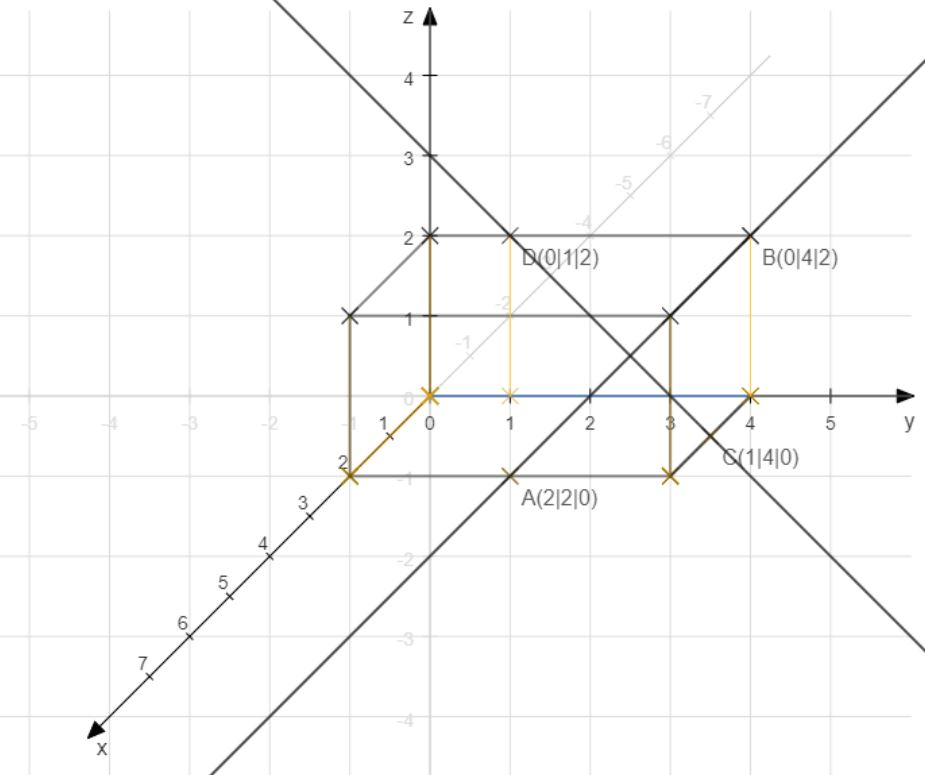
\includegraphics[scale=0.5]{Bilder/S65N9.jpg}
			\end{tabularx}\\
			\underline{\textbf{Frage}}: Schneiden sich die dargestellten Geraden?
			\par\noindent
			Zunächst stellen wir die Geraden \(g: \vec{x} = \vec{p} + r*\vec{u}\) durch A und B; \(h: \vec{x} = \vec{q} + t*\vec{v}\) durch C und D auf.\\
			\par\noindent
			\begin{tabularx}{\textwidth}{X|X}
				\(\vec{p} = \left(\begin{array}{c}2\\2\\0\end{array}\right)\) & \(\vec{p} = \left(\begin{array}{c}1\\4\\0\end{array}\right)\)\\
				\(\vec{u} = \vec{B} - \vec{A} =  \left(\begin{array}{c}-2\\2\\2\end{array}\right)\) & \(\vec{v} = \vec{D} - \vec{C} =  \left(\begin{array}{c}-1\\-3\\2\end{array}\right)\)\\
				\(g: \vec{x} = \left(\begin{array}{c}2\\2\\0\end{array}\right) + r*\left(\begin{array}{c}-2\\2\\2\end{array}\right)\) & \(h: \vec{x} = \left(\begin{array}{c}1\\4\\0\end{array}\right) + r*\left(\begin{array}{c}-1\\-3\\2\end{array}\right)\)
			\end{tabularx}
			Da wir wissen wollen, ob sich die Geraden schneiden, setzen wir \(g=h\).\\
			\begin{tabularx}{\textwidth}{rll}
				I & \(2-2r = 1 - 1t\) & \(|-1\ |:(-1)\)\\
				& \(-1 +2r = t\)\\
				II & \(2+2r = 4 - 3t\) &\\
				(*) & \(0 +2r = 0 + 2t\) & \(\Rightarrow r=t\)\\
			\end{tabularx}\\
			Wir setzen nun (*) zunächst in I ein.\\
			\begin{tabularx}{\textwidth}{rll}
				I & \(-1 +2t = t\) & \(|-t\ |+1\)\\
				& \(t = 1\)\\
				& \(\Rightarrow r = 1\)
			\end{tabularx}\\
			Anschließend prüfen wir mit II, ob unsere errechneten Werte für \(r\) und \(t\) stimmen.\\
			\begin{tabularx}{\textwidth}{rll}
				II & \(2+2*1 = 4 \neq 1 = 4 - 3*1\) & \(\lightning\)\\
			\end{tabularx}
			\(\Rightarrow\) Wir erhalten einen Widerspruch. Die Geraden haben somit \underline{\textbf{keinen}} Schnittpunkt.\\
		\end{framed}
	\end{worksheet}
\end{document}